
\begin{wrapfigure}{r}{0.4\textwidth}
    \begin{center}
        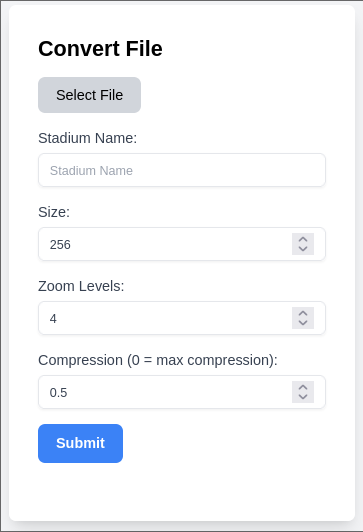
\includegraphics[scale=0.5]{pics/new_map_mask.png}
        \caption{New Map Mask}
        \label{fig:impl:mapgen}
    \end{center}
\end{wrapfigure}

A significant milestone in the project was the development of the map generation functionality. This feature enables the user to generate an empty seat plan, which relies on the map to serve as the basic visual representation of the venue. The map is interactive in the frontend, and the user can configure several key parameters:

\begin{itemize} 
    \item The venue plan 
    \item The name of the map 
    \item The size of each tile (default is 256x256px for most use cases) 
    \item The number of zoom levels 
    \item The image compression algorithm, which is a dropdown menu with the options: No Compression, Default Algorithm and Zopfli \end{itemize}

These configuration options are accessible under the "New Map" button, as depicted in Figure \ref{fig:impl:mapgen}.

The venue plan is always provided in SVG format, as the application does not support other file formats. To render the map, we use Leaflet, a JavaScript library designed for interactive maps. A Leaflet map is structured as a 3-dimensional pyramid of tiles, where each tile represents an image. The map's zoom dimension can be considered the "z-axis," while the horizontal and vertical axes correspond to the "x" and "y" axes of the map. Importantly, the x and y axes remain consistent across all zoom levels.

As a result, each tile is defined by a 3-dimensional coordinate in the map. These tiles are retrieved from an S3 bucket and processed by Leaflet in the frontend. The map's structure follows the form of a 3-dimensional pyramid with a square base, progressively expanding as the zoom level increases. The number of tiles per zoom level grows exponentially by a factor of two.

For a given zoom level \( z \), the number of tiles at that level is calculated as:
\[
\text{Number of tiles}(z) = 4^{(z-1)}
\]

The length of the side of the square base of the pyramid is:
\[
\text{Length of side}(z) = 2^{(z-1)}
\]

The total number of tiles is given by the sum:
\[
S(z) = \sum_{k=1}^{z} 4^{(k-1)} = \frac{4^z - 1}{3}
\]
As the number of zoom levels grows the number of tiles we need to process rises exponentially, and we reach a huge number of tiles very fast. For example, we already have 4095 256x256px images with 6 zoom levels.

\subsection{Step 1: Convert SVG to PNG}

The first step in generating this map structure is to convert the SVG file into a PNG image. This process is handled by the backend using the Batik image transcoder. Apache Batik is a robust, pure-Java library developed by the Apache Software Foundation for rendering, generating, and manipulating Scalable Vector Graphics (SVG). Batik provides various tools for tasks such as:

\begin{itemize} \item Rendering and dynamic modification of SVG files \item Transcoding SVG files into raster image formats (as done in this project) \item Transcoding Windows Metafiles to SVG \end{itemize}

The size of the image is determined by the current zoom level. The width and height are calculated based on the logic described earlier and implemented in the Kotlin code snippet in Listing \ref{lst:kotlin:dimensions}.

\begin{lstlisting}[language=Kotlin,caption=Image dimensions calculation,label=lst:kotlin:dimensions] 
Dimension(frameSize * 2.0.pow(zoomLevel).toInt(), frameSize * 2.0.pow(zoomLevel).toInt()) 
\end{lstlisting}

If the image is not square, it is centered within a square canvas, with the remaining area filled with white. The resulting image is then converted to PNG format and written to a Java ByteArrayOutputStream, which is used in the subsequent processing step.

\subsection{Step 2: Slicing the Image into Tiles}

In this step, the PNG image generated in the previous step is sliced into smaller tiles. The size of the tiles is determined by the user, with 256x256px being the default. Given that the image is always square and its dimensions are divisible by the tile size, the image can be split into an integer number of tiles without complications. 

The slicing process works by iterating through the image and extracting a sub-image of the specified tile size. This is done by calculating the appropriate coordinates for each tile and using the \texttt{Graphics.drawImage} method to copy the respective portion of the image into a new BufferedImage for each tile.

Here is the Kotlin code implementation for the slicing process:

\begin{lstlisting}[language=Kotlin,caption=Image Slicing Implementation,label=lst:kotlin:slicing]
val subImage = BufferedImage(sliceSize, sliceSize, BufferedImage.TYPE_INT_ARGB)
val graphics = subImage.createGraphics()
graphics.drawImage(image, 0, 0, sliceSize, sliceSize, x * sliceSize, y * sliceSize, (x + 1) * sliceSize, (y + 1) * sliceSize, null)
graphics.dispose()

\end{lstlisting}

In this code, \texttt{sliceSize} represents the size of each individual tile (e.g., 256x256px), and \texttt{x} and \texttt{y} are the coordinates of the current tile. The image is drawn on the \texttt{subImage} BufferedImage, which is a sub-region of the original image.

The resulting sub-images are saved as individual PNG files, each representing one tile of the map at the specified zoom level. These tiles are then going to be uploaded to the S3 bucket, so that the fronzend can fetch them as needed. By splitting the image into tiles, we can load and display the map interactively, only fetching the tiles that are currently in view. This tiling strategy is essential for efficient handling of large map layers at the later zoom levels.

LZ77 algorithm is a dictionary-based compression technique that replaces repeated occurrences of data with references to previous instances, reducing redundancy. Huffman coding, on the other hand, assigns shorter binary codes to more frequently occurring byte sequences, further optimizing storage efficiency. Together, these methods enable PNG files to achieve significant compression while maintaining full image fidelity.

\subsection{Step 3: Compression}

To optimize AWS costs and improve image loading speed in the frontend of the Ticketing project, images are compressed before being uploaded to the S3 bucket. However, this presents a challenge, as Solvistas requires PNG format for their project. Unlike lossy formats such as JPEG, which achieve smaller file sizes by discarding some image data, PNG is a lossless format, meaning it retains all original data. While this ensures sharp and clear images, it also results in larger file sizes, which can be problematic when numerous images are loaded from AWS in a web environment.


During the map generation process, users can choose from the following compression algorithms:

\begin{compactitem}
    
\item{}\textbf{None} – No compression applied (fastest processing time, largest file size).
\item{}\textbf{Default} – Standard compression using Deflate (balanced efficiency).
\item{}\textbf{Zopfli} – Advanced, high-efficiency compression (better compression rates, slower processing).
\end{compactitem}

The None option results in a 0\% compression rate, making it the fastest but least efficient choice.

For the other two compression options, we utilize the Pngtastic library, a lightweight, pure Java library with no dependencies. It provides a simple API for PNG manipulation, supporting both file size optimization and PNG image layering.

The Default option, uses the Deflate algorithm, which is used for as a base for many lossless compression algorithms, which combines LZ77 and Huffman coding.

\begin{compactitem}
\item{}\textbf{LZ77} is a dictionary-based compression method that reduces redundancy by replacing repeated sequences of data with references to earlier occurrences, thus minimizing file size without loss of quality.
\item{}\textbf{Huffman coding} optimizes storage efficiency by assigning shorter binary codes to frequently occurring byte sequences, further improving compression rates.
\end{compactitem}

Together, these methods enable PNG files to achieve significant compression while maintaining full image fidelity.

The Zopfli algorithm, developed by Google engineers Lode Vandevenne and Jyrki Alakuijala in 2013, offers an advanced, high-efficiency compression technique. While it still utilizes the Deflate algorithm, it applies exhaustive entropy modeling and shortest path search techniques to achieve a higher compression ratio than standard Deflate and zlib implementations. Zopfli achieves superior data compression by extensively analyzing different possible representations of the input data and selecting the most efficient encoding. By default, Zopfli performs 15 iterations to refine compression, though this can be adjusted for higher or lower processing times. Under standard settings, Zopfli output is typically 3–8\% smaller than zlib’s maximum compression, but it is approximately 80 times slower due to its computational intensity.

According to Google developers: \cite{ZopfliGoogleBlog}

\begin{quote}
    The smaller compressed size allows for better space utilization, faster data transmission, and lower web page load latencies. Furthermore, the smaller compressed size has additional benefits in mobile use, such as lower data transfer fees and reduced battery use.
\end{quote}

While Zopfli is significantly slower than standard Deflate or zlib, but this isn't a huge problem for this usecase, because time can be sacrificed once for the optimization and speed improvement for the user.

\subsubsection{Analysis of Compression Algorithms}

\begin{figure}
    \centering
    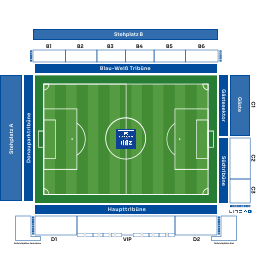
\includegraphics[scale=0.8]{pics/test_stadium.png}
    \caption{BW-Linz Stadium}
    \label{fig:impl:bw-stadium}
\end{figure}

By testing the compression algorithms within this application with different parameters, that range from the 3 algorithm, different maps and different number of zoom levels, we can see that Zopfli is the best option for the compression of the images, if the time is willing to be spent on compressing the data. All the test results are visualized in the following table, the image used for testing is the BW-Linz stadium \ref{fig:impl:bw-stadium}, which is an example taken out of production:


\begin{table}[h]
    \centering
    \begin{tabularx}{\textwidth}{|c|X|X|X|X|}
        \hline
        \textbf{Zoom Level} & \textbf{Size Before Compression (Bytes)} & \textbf{Size After Compression (Bytes)} & \textbf{Time Taken (ms)} & \textbf{Percent Saved} \\ \hline
        0 & 12148 & 12148 & 98 & 0\% \\ \hline
        1 & 28218 & 28218 & 243 & 0\% \\ \hline
        2 & 61540 & 61540 & 652 & 0\% \\ \hline
        3 & 131470 & 131470 & 1424 & 0\% \\ \hline
        4 & 289606 & 289606 & 2815 & 0\% \\ \hline
        5 & 700382 & 700382 & 7275 & 0\% \\ \hline
    \end{tabularx}
    \caption{Compression Results for NONE Compression Method}
    \label{tab:compression_none}
\end{table}

% Second Table
\begin{table}[h]
    \centering
    \begin{tabularx}{\textwidth}{|c|X|X|X|X|}
        \hline
        \textbf{Zoom Level} & \textbf{Size Before Compression (Bytes)} & \textbf{Size After Compression (Bytes)} & \textbf{Time Taken (ms)} & \textbf{Percent Saved} \\ \hline
        0 & 12148 & 10043 & 533 & 17.47\% \\ \hline
        1 & 28218 & 24710 & 1477 & 12.43\% \\ \hline
        2 & 61540 & 58638 & 4534 & 4.99\% \\ \hline
        3 & 131470 & 131226 & 14397 & 0.19\% \\ \hline
        4 & 289606 & 289134 & 51388 & 0.16\% \\ \hline
        5 & 700382 & 699310 & 180054 & 0.15\% \\ \hline
    \end{tabularx}
    \caption{Conversion Results for DEFAULT Compression Method}
    \label{tab:compression_default}
\end{table}

% Zopfli Compression Table with Fictional Data
\begin{table}[h]
    \centering
    \begin{tabularx}{\textwidth}{|c|X|X|X|X|}
        \hline
        \textbf{Zoom Level} & \textbf{Size Before Compression (Bytes)} & \textbf{Size After Compression (Bytes)} & \textbf{Time Taken (ms)} & \textbf{Percent Saved} \\ \hline
        0 & 12148 & 9745 & 13179 & 19.73\% \\ \hline
        1 & 28218 & 23343 & 35591 & 17.29\% \\ \hline
        2 & 61540 & 54519 & 111915 & 11.41\% \\ \hline
        3 & 131470 & 119405 & 363794 & 9.18\% \\ \hline
        4 & 289606 & 266976 & 1166758 & 7.82\% \\ \hline
        5 & 700382 & 658512 & 3004721 & 5.98\% \\ \hline
    \end{tabularx}
    \caption{Conversion Results for ZOPFLI Compression Method}
    \label{tab:compression_zopfli}
\end{table}

% Summary Table
\begin{table}[h]
    \centering
    \begin{tabular}{|p{7cm}|p{2.1cm}|p{2.1cm}|p{2.1cm}|}
        \hline
        \textbf{Compression Method} & \textbf{NONE} & \textbf{DEFAULT} & \textbf{ZOPFLI} \\ \hline
        \textbf{Total Size Before Compression (Bytes)} & 1223364 & 1223364 & 1223364 \\ \hline
        \textbf{Total Size After Compression (Bytes)} & 1223364 & 1213061 & 1132500 \\ \hline
        \textbf{Total Bytes Saved (Bytes)} & 0 & 10303 & 90964 \\ \hline
        \textbf{Total Percent Saved} & \textbf{0\%} & \textbf{0.84\%} & \textbf{7.44\%} \\ \hline
        \textbf{Total Time Taken (ms)} & 7519 & 195929 & 4696028 \\ \hline
        \textbf{Total Time Taken (min)} & 0.13 & 3.27 & 78.27 \\ \hline
    \end{tabular}
    \caption{Summary of Conversion Results}
    \label{tab:summary_compression}
\end{table}

To ensure that this test data is viable, the calculation has been computed with 4 dedicated processors, that were configured like this as java vm options:

\texttt{-XX:ActiveProcessorCount=4}

As you can observe in the summary table \ref{tab:summary_compression} and as expected has amazing compression but is a very time intensive process. In the end we save 6.6\% more than the default algorithm, but it takes ~24 times longer, and waiting times for over an hour should be calculated when using the algorithm. This is a trade-off that has to be considered. Because this would only be a one time process the decision could fall for Zopfli, but in comparison to the total 90964 Bytes (88.83=KiB) saved this is still not a huge amount of data saved, when considering the time taken. In the end all the data produced is not very large, so the operator has to decide if the time is worth the saved data. If the time and resources don't want to be spent for such a low storage and performance improvement, the default algorithm is still a good choice, because a waiting period of 3 minutes 16 seconds is still acceptable for a small bit of optimization. As mentioned previously it's very important, that the user can decide what algorithm should be used because of lots of factors. When the program is hosted on an external cloud provider with dynamic cost calculation, the user probably doesn't want to spend the extra money for the Zopfli algorithm, because the cost for the extra time could be higher than the saved money for the storage. If the program is executed locally or servers that have enough free resources the Zopfli algorithm is an excelent choice.

Another significant decision during development was whether to compress the images before or after the slicing process. Ultimately, we decided to compress the images before slicing them into tiles. This approach was favored for several reasons.

Compressing the entire image as a whole is generally more efficient than compressing individual tiles. Compression algorithms benefit from analyzing the entire dataset, allowing them to identify and eliminate redundancies more effectively. When an image is compressed in its entirety, the algorithm can exploit correlations and patterns that might not be as apparent when processing smaller segments. This leads to a better overall compression ratio, resulting in reduced file sizes without sacrificing quality.

Had we chosen to first slice the images and then compress the individual tiles in parallel, we would have faced potential issues with resource contention. In such a scenario, multiple instances of the Zopfli compression algorithm could run simultaneously, each consuming considerable CPU cycles and memory. Given Zopfli’s high computational demands, this could overwhelm the heap space, leading to memory exhaustion or, at the very least, severely impacting overall system performance. In extreme cases, excessive resource usage could degrade the performance of the entire operating system, causing bottlenecks and slowdowns.

\subsection{Step 4: Uploading Tiles to S3}

The final step in the map generation process involves uploading the generated tiles to an Amazon S3 bucket. This is achieved using the AWS SDK for Java, which provides a robust and efficient way to interact with AWS services. The SDK allows us to create an S3 client, which facilitates seamless communication with the S3 bucket. The only required configuration parameters for the client are the AWS region (set to eu-central-1 in our case), the access key, and the secret key. Once configured, as demonstrated in Listing \ref{lst:kotlin:s3client}, the S3Client instance provides a range of operations, including putObject, getObject, and listObjectsV2, among others.

\begin{lstlisting}[language=Kotlin,caption=Configuring the S3 Client,label=lst:kotlin:s3client]
@ConfigurationProperties(prefix = "aws")
data class S3Config @ConstructorBinding constructor(
    val awsRegion: String,
    val accessKey: String,
    val secretKey: String
){
    @Bean(destroyMethod = "close")
    fun s3Client() : S3Client {
        return S3Client
            .builder()
            .overrideConfiguration(ClientOverrideConfiguration.builder()
                .apiCallTimeout(Duration.ofSeconds(10)).build()
            )
            .region(Region.regions()
                .find { region -> region.toString() == awsRegion }
            )
            .credentialsProvider(
                StaticCredentialsProvider.create(
                    AwsBasicCredentials.create(accessKey, secretKey)
                )
            )
            .build()
}
\end{lstlisting}

The configuration is managed using the @ConfigurationProperties(prefix = ``aws'') annotation, which enables automatic injection of required properties. These values—defined in the primary constructor with @ConstructorBinding—are retrieved from an external properties file under the aws prefix. This approach ensures that configuration values remain externalized rather than hardcoded, making it easier to switch between environments such as development, testing, and production. The relevant configuration in application.yml is illustrated in Listing \ref{lst:yaml:aws}.
\begin{lstlisting}[language=Yaml, caption=AWS Configuration in application.yml, label=lst:yaml:aws]
aws:
    awsRegion: ${AWS_REGION:eu-central-1}
    access-key: ${AWS_ACCESS_KEY}
    secret-key: ${AWS_SECRET_KEY}
\end{lstlisting}

By using environment variables for sensitive credentials, we enhance security while maintaining flexibility in deployment configurations.
The SDK’s S3Client.builder() method is used to instantiate and configure the client with the required credentials and region settings. Because the client is defined as a Spring bean, it can be easily injected into any class requiring interaction with the S3 bucket. This is a key advantage in Spring-based applications, as it promotes modularity and maintainability. Unlike in Quarkus, where dependency injection is handled differently, Spring allows defining such functions as beans and seamlessly injecting them where necessary.

The name provided by the user doesn't have any major restrictions for special characters, that's because the customer shouldn't be bothered with technical restrictions. They should be able to choose the name they want. Technically there are still some restrictions. The name provided by the user will be used in two situations, that have limitations. 
\begin{compactenum}
    \item Directory names in the S3 buckets
    \item Path in our URL frontend for editor page
\end{compactenum}

S3 looks like a standard file system, but actually it's not, and therefore the name for the ``directory'' doesn't have huge limitations. 

Normally data in an Amazon S3 bucket, is stored in a flat structure instead of a hierarchy one as seen in standard file systems. Amazon still supports the organization of data like in file systems. This is done by giving all the grouped objects a shared string prefix. The prefix is therefore the folder name. The data, is actually still stored in a flat structure, but it's visualized like folders in the Amazon S3 console.

The second place where name is utilized, is the URL path in the frontend. This is a bit more restricted, because it's part of the URL and therefore some characters could lead to errors. These following characters are reserved and can't be used in the URL path: \texttt{/\&?=:\%}. When these are used this leads to errors. This is why we prepare the name for the URL path by replacing these characters with an underscore. To still give the user the requested name, we store the original name in our database as well as the prepared name. The original name is only used for displaying purposes in the frontend.

After executing all of these steps, they have to be repeated for each zoom level asked for. 

\subsection{Optimizations \& Memory}

This process involves repetitive and computationally demanding tasks such as image slicing, format conversion, and compression, making it well-suited for multi-threading. However, parallel execution introduces challenges, particularly with Java heap space management. During slicing and compression, a large amount of data is stored in memory at the same time. This includes both the upscaled source image and the processed image tiles, leading to high memory usage. At higher zoom levels, storage requirements can reach several gigabytes, potentially exceeding the allocated heap space and causing OutOfMemoryError exceptions.

To address this, the Java heap size can be manually adjusted using:

\texttt{java -Xmx6g seatgen}

This increases the maximum heap allocation to \texttt{6 GB}, allowing for more memory-intensive operations. On \texttt{32-bit} systems, the heap size should not exceed 2 GB, as Java will reject larger values and fail with an invalid memory allocation error.

While manually increasing the heap size is a possible solution, we wanted to ensure that the application runs efficiently without requiring users to adjust memory settings, although it's recommended when planning to use the Zopfli algorithm. To achieve this, we limited the number of parallel threads to prevent excessive memory usage and placed a cap on the maximum zoom level. At higher zoom levels, the processing demands grow exponentially, making it impractical to handle them within a Java-based backend. If future requirements necessitate even higher zoom levels, a more efficient approach could involve using a language like C, Rust, or Python, which offer better memory management for such intensive operations. However, since the company currently does not require zoom levels beyond level 6, this remains an optimization for future development.
Leveraging Kotlin Coroutines for Concurrency

To further optimize the performance and manage concurrency effectively, we utilized Kotlin coroutines. Coroutines provide a lightweight and efficient way to handle asynchronous programming, allowing us to perform tasks like image slicing, compression, and uploading in a non-blocking manner. Unlike traditional threads, coroutines are more memory-efficient and can be launched in large numbers without overwhelming the system.

For example, during the slicing and compression phases, we used coroutines to parallelize tasks such as processing individual rows of tiles. This allowed us to maximize CPU utilization while keeping memory usage under control. By structuring the workflow with coroutines, we were able to ensure that tasks like garbage collection and memory cleanup could be triggered at appropriate intervals, preventing memory leaks and excessive heap usage.

The limitation logic for the number of threads for parallelization is based on the algorithm used for compression, because for Zopfli, this is the most memory-critical part. When using Zopfli, which is particularly memory-intensive, we limit the parallelism to a single thread during the compression phase. This approach ensures that we do not overwhelm the system's memory, allowing for more efficient processing. However, the slicing of image rows can still be executed with a maximum of four coroutines running concurrently, striking a balance between performance and resource usage. For the DEFAULT compression algorithm, we adopt a more aggressive approach, utilizing half of the available threads. This strikes a balance between efficient processing and maintaining manageable memory consumption. In scenarios where no compression methods are applied, we allow for the full use of the available processor threads. By limiting the number of concurrent coroutines when using Zopfli or the default algorithm, we mitigate the risk of exceeding heap space during high-demand processes like compression and slicing.

After each complete calculated zoom level, a garbage collection is triggered to free up memory that is no longer needed. This is done by calling the \texttt{System.gc()} method, which is a hint to the JVM to run the garbage collector. While this is not a guarantee that the garbage collector will run, it provides a good hint for the JVM to do so.

Because of memory problems, we also decided not to upload all the data of the images when everything is finished. Instead, we upload the data for each row of tiles as soon as it is completed. This approach provides a good balance between memory usage and efficiency, as we avoid storing all the data in memory while waiting for other rows to be computed. Uploading the tiles in the form of rows is also more efficient than uploading every tile individually to the S3 bucket, as it reduces the overhead significantly. For example, on zoom level 6, we only need to make 63 requests instead of 1365 requests.